%%%%%%%%%%%%%%%%%%%%%%%%%%%%%%%%%%%%%%%%%
% Tutorial
% LaTeX Template
% Version 1.0 (09/27/17)
%
% Author:
% Ben Roose (ben.roose@wichita.edu)
%
% Original template author:
% Adam Glesser (adamglesser@gmail.com)
% www.LaTeXTemplates.com
%
% License:
% CC BY-NC-SA 3.0 (http://creativecommons.org/licenses/by-nc-sa/3.0/)
%
%%%%%%%%%%%%%%%%%%%%%%%%%%%%%%%%%%%%%%%%%

\documentclass[12pt]{article}

\usepackage{graphicx} %Allow import of images
\graphicspath{ {images/} } % Relative path to images directory
\usepackage[margin=1in]{geometry} % Required to make the margins smaller to fit more content on each page
\usepackage[linkcolor=blue]{hyperref} % Required to create hyperlinks to questions from elsewhere in the document
\hypersetup{pdfborder={0 0 0}, colorlinks=true, urlcolor=blue} % Specify a color for hyperlinks
\usepackage{todonotes} % Required for the boxes that questions appear in
\usepackage{tocloft} % Required to give customize the table of contents to display questions
\usepackage{microtype} % Slightly tweak font spacing for aesthetics
\usepackage{palatino} % Use the Palatino font

\setlength\parindent{0pt} % Removes all indentation from paragraphs

% Create and define the list of questions
\newlistof{questions}{faq}{\large FAQ for remote access into cslab Linux environment}
% This creates a new table of contents-like environment that will output a file with extension .faq
\setlength\cftbeforefaqtitleskip{3em} % Adjusts the vertical space between the title and subtitle
\setlength\cftafterfaqtitleskip{1em} % Adjusts the vertical space between the subtitle and the first question
\setlength\cftparskip{.3em} % Adjusts the vertical space between questions in the list of questions

% Create the command used for questions
\newcommand{\question}[1] % This is what you will use to create a new question
{
\refstepcounter{questions} % Increases the questions counter, this can be referenced anywhere with \thequestions
\hfill
\goodbreak
\par\noindent % Creates a new unindented paragraph
\phantomsection % Needed for hyperref compatibility with the \addcontensline command
\addcontentsline{faq}{questions}{#1} % Adds the question to the list of questions
\todo[inline, color=green!40]{\textbf{#1}} % Uses the todonotes package to create a fancy box to put the question
%\vspace{0.5em} % White space after the question before the start of the answer
}

% Uncomment the line below to get rid of the trailing dots in the table of contents
%\renewcommand{\cftdot}{}

% Uncomment the two lines below to get rid of the numbers in the table of contents
%\let\Contentsline\contentsline
%\renewcommand\contentsline[3]{\Contentsline{#1}{#2}{}}

\begin{document}

%----------------------------------------------------------------------------------------
%	TITLE AND LIST OF QUESTIONS
%----------------------------------------------------------------------------------------

\begin{center}
\Huge{\bf \emph{EECS Tutorial: cslab Linux Environment}} % Main title
\end{center}

\listofquestions % This prints the subtitle and a list of all of your questions
\bigskip % Create a gap between list and first question

\newpage % Comment this if you would like your questions and answers to start immediately after table of questions

%----------------------------------------------------------------------------------------
%	QUESTIONS AND ANSWERS
%----------------------------------------------------------------------------------------

\question{How do I access the cslab Linux environment via a web-browser?}\label{guac_login}

\begin{enumerate}
\item Open your favorite HTML5 compatible web-browser. To test the compatibility of your browser go to \href{https://html5test.com/}{html5test.com}
\item In your browser go to \href{https://cslab-gateway.cs.wichita.edu/}{cslab-gateway.cs.wichita.edu}
\item At the login screen enter your myWSU ID and password and you will be presented with the \textit{Apache Guacamole} home screen.
\begin{figure}[h]
%\caption{Example of \textit{Guacamole} home screen when you first log in}
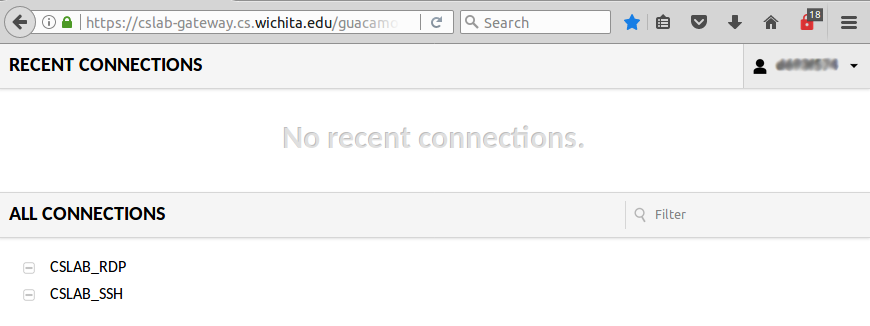
\includegraphics[width=\linewidth]{screenshot_cslab_initial_homescreen}
\centering
\end{figure}
\item To connect into an LXDE graphical RDP desktop session for working on programming assignments click on \texttt{CSLAB\_RDP}.
\item To connect into a command-line SSH terminal session for working on programming assignments click on \texttt{CSLAB\_SSH}.
\item When you next log into \href{https://cslab-gateway.cs.wichita.edu/}{cslab-gateway.cs.wichita.edu} the \textit{Apache Guacamole} home screen will show clickable thumbnails of your recent connections.
\item To log out of \textit{Guacamole} from the home screen, click on your \texttt{myWSU\_ID} at the top right. This drop-down list also enables you to open the \texttt{Settings} menu which includes displaying an on-screen keyboard for mobile devices.

\begin{figure}[h]
%\caption{Example of \textit{Guacamole} home screen with recent connection thumbnails}
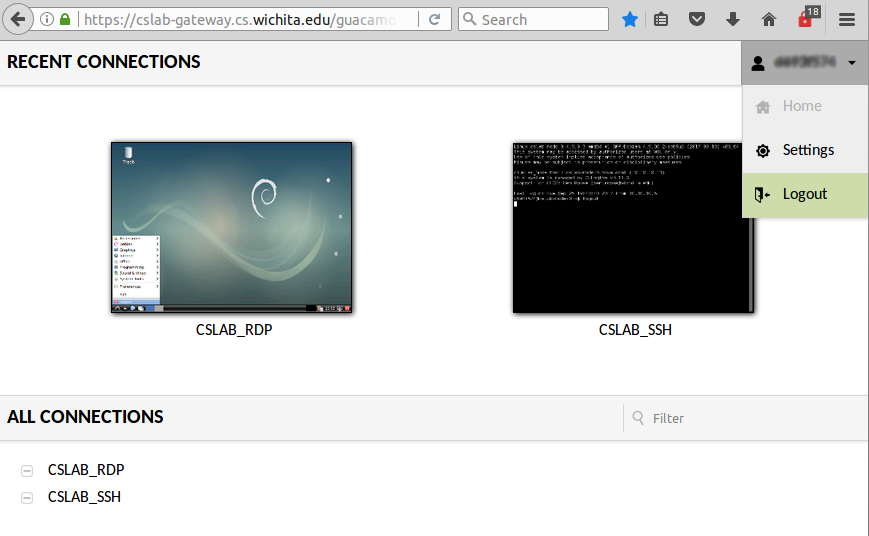
\includegraphics[width=\linewidth]{screenshot_cslab_logout_homescreen}
\centering
\end{figure}

\item During your initial connection into an RDP desktop session, occasionally you may see a policykit error message pop-up window. This is a known software bug which is being worked on. Clicking the OK button will close the error and it should not affect the rest of your login session.
\item To open/close the \textit{Guacamole} menu sidebar while in the cslab environment press the key combination \textbf{Ctrl+Alt+Shift}. The \textit{Guacamole} menu sidebar enables you to log out, disconnect, change settings, upload/download files, and use a remote clipboard.
\item For further help on using the \textit{Guacamole} interface go to \href{https://guacamole.incubator.apache.org/doc/gug/using-guacamole.html}{Using Guacamole Guide}
\end{enumerate}
\textbf{NOTE: When you finish your work session, please make sure to logout from your connection within the cslab environment:
\begin{itemize}
\item by using the \textit{Guacamole} menu sidebar,
\item by using the [logout] menu item or [logout] taskbar button within the RDP desktop session, or
\item by typing \texttt{exit} or pressing \textbf{Ctl+D} within the SSH terminal session.
\end{itemize}}

%------------------------------------------------
%% \newpage

\question{What software is available within the cslab Linux environment?}\label{cslab_software}

The cslab environment gives you both graphical and command-line Linux tools for writing, compiling, and debugging your CS programming class assignments. The Linux operating system running in cslab is Debian 9 (stretch) with a default LXDE desktop and Bash shell. Software tools/packages installed on the cslab-nodes include:
\begin{itemize}
\item Text and code editors: leafpad, nano, vim, and emacs.
\item Integrated development environments (IDE): atom, geany, and eclipse.
\item Compiling tools: GNU C compiler (gcc), g++, make, prolog, perl, python, and java.
\item Debugging tools: GNU debugger (gdb) and data display debugger (ddd).
\item Latex tools: pdflatex, texlive, and texmaker.
\item Version control tools: git and subversion.
\item GUI terminal emulators: terminator, lxterminal, and xterm.
\item CLI terminal multiplexers: screen and tmux.
\end{itemize}
To check if a specific software package or version is installed within the cslab-nodes, connect into the SSH terminal session or open a terminal emulator in the RDP desktop session and type:
\begin{verbatim}
apt list --installed specify_package_name_here
\end{verbatim}

If a Linux software package is not installed within the cslab Linux environment which you require to complete your class assignment, then please ask your instructor whether this package can be installed for you by the EECS systems administrator.

\bigskip

\textbf{Do not attempt to install any software packages yourself!}

%------------------------------------------------

\question{How do I copy text within the cslab Linux environment? }\label{text_copying}

\subsection*{Copying text from your local computer to the remote environment:}
\begin{enumerate}
\item Copy the required text to the clipboard within your local computer application using your preferred method of copying, i.e. \textbf{Ctrl+C}.
\item Within the cslab environment in your browser, open the \textit{Guacamole} menu sidebar by pressing the key combination \textbf{Ctrl+Alt+Shift}.
\item Paste the copied text to the remote \textit{Guacamole} [Clipboard] field using your preferred method, i.e. \textbf{Ctrl+V}.
\item Close the \textit{Guacamole} menu sidebar by pressing the key combination \textbf{Ctrl+Alt+Shift}.
\item Within the RDP desktop session, any text shown in the \textit{Guacamole} [Clipboard] can be pasted into a remote cslab application by normal methods, i.e. \textbf{Ctrl+V}.
\item Within the SSH terminal session, text in the \textit{Guacamole} [Clipboard] can be pasted into the terminal by right-clicking on the browser window with your mouse or by pressing the key combination \textbf{Ctrl+Shift+V}.
\end{enumerate}

\subsection*{Copying text from the remote environment to your local computer:}
\begin{enumerate}
\item Within the RDP desktop session, text can be cut or copied from any cslab application by normal cut/copy methods, i.e. \textbf{Ctrl+C}.
\item Within the SSH terminal session, text to be copied is "highlighted" using the mouse.
\item Open the \textit{Guacamole} menu sidebar by pressing the key combination \textbf{Ctrl+Alt+Shift}.
\item The copied or "highlighted" text will appear in the remote \textit{Guacamole} [Clipboard] and can then be selected and copied to your local computer clipboard, i.e. \textbf{Ctrl+C}.
\item Close the \textit{Guacamole} menu sidebar by pressing the key combination \textbf{Ctrl+Alt+Shift}.
\end{enumerate}

%------------------------------------------------

\question{How do I download/upload files within the cslab Linux environment? }\label{file_copying}

\subsection*{Using guacctl/guacget to download a file:}
\begin{itemize}
\item Within the SSH terminal session, you can use the \textit{Guacamole terminal session control utility (guacctl)} for downloading files. To download a file from the SSH terminal session to your local computer via the web-browser type:
\begin{verbatim}
guacget file_to_be_downloaded
\end{verbatim}
\item \texttt{guacget} is an alias for the command \texttt{guacctl --download}. To see all the option flags available for this command type \texttt{guacctl}.
\item \textbf{NOTE: \texttt{guacget} only works in SSH terminal sessions. \texttt{guacget} does not work in RDP desktop sessions.}
\end{itemize}

\subsection*{Drag-and-drop to upload a file:}
\begin{itemize}
\item You can drag-and-drop a file from your local computer onto the cslab web-browser window. This can be used in both RDP desktop and SSH terminal sessions.
\item By default the file is uploaded into your user home directory on the remote cslab-node.
\item You can set a custom destination directory for future uploaded files when using drag-and-drop by typing:
\begin{verbatim}
guacctl -s custom_upload_directory
\end{verbatim}
\end{itemize}

\subsection*{\textit{Guacamole} file browser to upload or download a file:}
\begin{enumerate}
\item Open the \textit{Guacamole} menu sidebar by pressing the key combination \textbf{Ctrl+Alt+Shift}.
\item Click on the disk drive icon under [Devices] to open a file browser of the remote cslab-node.
\item Browse to your user home directory on the remote server. You can then browse to subdirectories within your user home. Your home directory full path on the remote cslab-node will look like the following:
\begin{verbatim}
/opt/homes/stu##/your_myWSU_id/
\end{verbatim}
\item If you are unsure where your home directory is located on the remote cslab-node, in a terminal or in the SSH terminal session type \texttt{pwd} to show you the full path of your present working directory.
\item Downloads are initiated by double-clicking on any file shown, while uploads are initiated by clicking the [Upload Files] button. Clicking [Upload Files] will open a file browsing dialog where you can choose one or more files from your local computer, ultimately uploading the selected files to the directory currently displayed within the remote cslab-node file browser.
\item Close the \textit{Guacamole} menu sidebar by pressing the key combination \textbf{Ctrl+Alt+Shift}.
\end{enumerate}

%------------------------------------------------

\question{Can I open multiple browser tabs/windows into the cslab Linux environment? }\label{multiple_tabs}

\begin{itemize}
\item A restriction within the RDP software only allows a single connection per user, which means you can view the remote RDP desktop session from only one web-browser tab/window at a time. If you attempt to open more than one web-browser tab/window and connect to multiple RDP desktop sessions, then the gateway will disconnect from one tab and reconnect in another tab.
\item A restriction within the SSH software allows a maximum of six concurrent connections per user, which means you can open up to six web-browser tabs/windows into remote SSH terminal sessions at the same time. Each open SSH terminal session tab/window will run a separate command-line shell instance on the same remote cslab-node.
\item You can use the \texttt{tmux} or \texttt{screen} terminal multiplexer commands to run multiple command-line shells concurrently in the same SSH session tab/window.
\item You can open one web-browser tab/window to connect to a graphical RDP desktop session and open additional tabs/windows to connect to SSH terminal sessions concurrently. However, the \textit{Apache Guacamole} system cannot guarantee that your RDP desktop session and your SSH terminal session(s) will connect to the same remote cslab-node.
\end{itemize}

%------------------------------------------------

\question{How do I access the cslab Linux environment on port 22 via an SSH client?}\label{ssh_client}

\textbf{Please only connect directly into the cslab environment with an SSH client if you have previous experience in using SSH and the Linux command-line. If you are new to Linux, please use the \hyperref[guac_login]{\textit{Guacamole} web-browser interface}.}

\subsection*{Using \textit{OpenSSH} client on Linux or Mac OSX:}
\begin{enumerate}
  \item Add the following host entry into your local user \texttt{ $\sim$/.ssh/config} file:
\end{enumerate}

\begin{verbatim}
Host cslab cslab-last cslab.cs.wichita.edu cslab-last.cs.wichita.edu
  ProxyCommand ssh your_mywsu_id@cslab-bastion.cs.wichita.edu ballast %h
  HostKeyAlias cslab.cs.wichita.edu
  User your_mywsu_id
\end{verbatim}
\begin{enumerate}
\setcounter{enumi}{1}
\item In a local CLI terminal connect to the cslab Linux environment by typing
\begin{verbatim}
ssh cslab
\end{verbatim}
\item The first time you connect to the cslab environment using SSH, you will be asked to confirm the authenticity of each SSH remote host, i.e.
\begin{verbatim}
The authenticity of host 'cslab.cs.wichita.edu' can't be established.
ECDSA key fingerprint is [SHA256 hash value].
Are you sure you want to continue connecting (yes/no)?
\end{verbatim}

Ensure the cslab-bastion and cslab host key fingerprints match one of the following before typing yes:
\begin{verbatim}
RSA key fingerprint is
SHA256:0CUyGZAYMdOd8vTOK3AtM2XTX3lMaGA2NP73rR7s6Ns.
DSA key fingerprint is
SHA256:7zW122xr+aoBb5yiRI96nvdx8Ml07qLKHYwG2Wu6jIM.
ECDSA key fingerprint is
SHA256:X6dBKj4sqYYPWol6MXSQvGhpIQ6qBxh7mBQhnSw8n64.
\end{verbatim}

\item You will be prompted twice to enter your myWSU password, once for the cslab-bastion (SSH jumphost) and once for the cslab-node.
\item If the SSH connection completed successfully, then you will be presented with a standard shell prompt:

\texttt{your\_my\_wsuid@cslab-node-\#:$\sim$\$}
\end{enumerate}

\textbf{NOTE: If you are accessing cslab via SSH on WSU campus, ensure you are connected to ``WSU Secure'' wireless network or using an Ethernet connected computer. ``WSU Guest'' wireless network prohibits port 22 connections and will fail to connect.}


%------------------------------------------------

\question{How do I use graphical (GUI) applications in cslab via an SSH client?}\label{x11_forwarding}

\subsection*{Using \textit{OpenSSH} client with X11 forwarding on Linux or Mac OSX:}
\begin{itemize}
\item Ensure you have followed the directions in \hyperref[ssh_client]{using \textit{OpenSSH} client} first.
\item SSH allows for graphical applications to run on a local computer from the remote cslab Linux environment using X11 forwarding.
\item To use X11 forwarding on a per session basis append the \texttt{-X} option flag to your SSH command, i.e.
\begin{verbatim}
ssh -X cslab
\end{verbatim}
\item To always use X11 forwarding for connections to cslab, instead of using the \texttt{-X} option flag, add the following line to the \texttt{Host cslab cslab-last} entry in your \texttt{ $\sim$/.ssh/config} file:
\begin{verbatim}
  ForwardX11 yes
\end{verbatim}
\item If you are using Mac OSX, then you may need to install XQuartz before using X11 forwarding. Download \href{https://www.xquartz.org}{XQuartz for Mac} and install the software package.
\end{itemize} 

%------------------------------------------------

\question{How do I copy files from/to the cslab Linux environment via an SSH client?}\label{scp_copying}

\subsection*{Using \textit{OpenSSH} client on Linux or Mac OSX:}
\begin{itemize}
\item Ensure you have followed the directions in \hyperref[ssh_client]{using \textit{OpenSSH} client} first.
\item To copy a file from your local computer to your user home directory on cslab using Secure Copy (SCP), type

\texttt{scp local\_filename\_or\_path cslab:$\sim$}

\item To copy a file from your user home directory on cslab to a local directory on your local computer, type

\texttt{scp cslab:$\sim$/remote\_filename\_or\_path local\_directory}
\end{itemize}

%------------------------------------------------

\question{How do I access the last accessed cslab-node via an SSH client?}\label{ssh -last}

\begin{itemize}
\item When connecting to the cslab Linux environment using \texttt{ssh cslab}, the ballast load-balancer will redirect you to one of the least used cslab-nodes at time of connection. Since load-balancing is calculated by ballast on a one minute cycle, you may not be redirected to the same cslab-node the next time you connect into cslab via SSH.
\item To connect to the last cslab-node you previously accessed via the load-balancer, you can append \texttt{-last} to the SSH command, i.e
\begin{verbatim}
ssh cslab-last
\end{verbatim}
\item \textbf{NOTE: All cslab-nodes automatically reboot every night between 2am and 3am. Any processes left running on a node will be killed.} 
\end{itemize} 

%------------------------------------------------

\end{document}
